\documentclass[11pt, twoside, reqno]{book}
\usepackage{amssymb, amsthm, amsmath, amsfonts}
\usepackage{graphicx}
\usepackage{color}
\usepackage{hyperref}
\usepackage{verbatim}
\usepackage[toc,page]{appendix}
\usepackage{listings}
\usepackage{float}
\usepackage{csvsimple}
\appendixpageoff

\usepackage{bardtex}

%The following optional command allows for a change in the method of inputting the bibliography.  The options are amsrefs'' and bibtex."  If the command is not used, the default is amsrefs.''  The bibliographic entries given at the end of this file are in the amsrefs format; a different format is needed for bibtex.  See the manual for details about the bibliography.

\styleoption{seniorproject}

%Your macros, if you have any.
\usepackage{color}
\definecolor{codegreen}{rgb}{0,0.6,0}
\definecolor{codegray}{rgb}{0.5,0.5,0.5}
\definecolor{codepurple}{rgb}{0.58,0,0.82}
\definecolor{backcolour}{rgb}{0.95,0.95,0.92}
 
\lstdefinestyle{mystyle}{
    backgroundcolor=\color{backcolour},   
    commentstyle=\color{codegreen},
    keywordstyle=\color{magenta},
    numberstyle=\tiny\color{codegray},
    stringstyle=\color{codepurple},
    basicstyle=\footnotesize,
    breakatwhitespace=false,         
    breaklines=true,                 
    captionpos=b,                    
    keepspaces=true,                 
    numbers=left,                    
    numbersep=5pt,                  
    showspaces=false,                
    showstringspaces=false,
    showtabs=false,                  
    tabsize=2
}
 
\lstset{style=mystyle}


\begin{document}

\titlepg{Predicting How People Vote From How They Tweet}{Rao Vinnakota}
    {May}{2019}

\abstr

In 2016 Donald Trump stunned the nation and not a single pollster predicted the outcome. For the last few decades, pollsters have relied on phone banking as their main source of information. There is reason to believe that this method does not present the complete picture it once did due to several factors--less landline usage, a younger and more active electorate, and the rise of social media. Social media specifically has grown in prominence and become a forum for political debate. This project quantitatively analyzes political twitter data and leverages machine learning techniques such as Naive-Bayes to model election results. Early results are promising, and a true evaluation of the model will come from testing in future elections. 

\tableofcontents

\dedic

Text of dedication.

\acknowl

Text of acknowledgments.

\startmain

%%%%%%%%%%%%%%%%%INTRODUCTION%%%%%%%%%%%%%%%%%%%%%%%%%

\intro
\hspace{0.2in}Donald Trump stunned the world when he was elected President of the United States. Trump ran an unorthodox campaign, specifically in regards to his use of social media. Trump used accounts on Twitter and Facebook as a voice to attack candidates, disseminate campaign information, and engage with voters. 

Public polling in 2016 didn’t predict the upset. In fact, it didn’t come particularly close. The latest tracking polls before election day showed Clinton in the lead with a margin of anywhere from +1 to +6. Most pollsters believed that Trump would sweep strictly conservative areas, but Clinton would every state that really mattered. Obviously, that didn’t happen

If you look through tweets following the election, Trump supporters claimed that victory was inevitable, and that Trump’s social media interaction demonstrated it. true? Was Trump’s potential victory present on social media for people to see? 

That is idea my senior project explore. Can you mathematically evaluate opinions on social media to predict voting trends. I will gather tweets pertaining to the 2018 midterm elections and use the sentiment expressed in those tweets and attempt to predict voting results. 


\section{Political Polling - A Short Overview}
\hspace{0.2in} The earliest iteration of polling was a straw poll conducted in Harrisburg, Pennsylvania which showed Andrew Jackson leading John Quincy Adams in the 1824 Presidential Election. Journalists from The \textit{Harrisburg Pennsylvanian} asked local voters which they preferred. Jackson winning both the polls and the election created legitimized the poll. Polls continued to be local until the early 20th century when Literary Digest sent out postcards to reader asking for their pick of the presidential election. The Literary Digest correctly predicted 5 straight elections and opinion polls reached the national stage. 

In the advertising boom of post-World War II, most polling shifted to telecommunications. With telephones, there was an ability to reach a wider audience, ask deeper questions. Pollsters could now build a profile of a voter, and forecast more accurate results. Accompanying the advance in polling was a focus on sampling. Pollsters couldn’t call every single house in the United States. Instead, groups of people or “samples” that would accurately represent the country were called. Responses from the sample were extrapolated to cover the whole. 

Today, the digital age and social media have made polling’s barrier of entry low. A short scroll through Twitter will show hundreds of “opinion polls”. Youtube videos’ likes and dislikes function as an informal poll. The Algorithm will often promote videos that are more “well-liked”. But, professional political polling is still done along the same lines. A population is sampled, called, and profiled. Profiling technique has improved. Today, forecasters like 538’s Nate Silver, will build complex profiles of voters in various regions. But, the source of the information and the method of obtaining the information remains the same. 

\section{Social Media, Twitter, and Politics}
\hspace{0.2in}The internet’s first foray into politics was in 2008. Barack Obama established that it was acceptable for a candidate to leverage the internet as a resource, using the internet as a tool for both message and money. The website MyBarackObama.com helped Obama set records in grassroot donations and mobilizations. 

Social websites from the forums of the early 2000s to social media platforms that are popular today are the most visited websites on the internet. These forums encourage conversation, including the discussion of politics. Especially for younger voters who don’t own any landlines, these forums are the few places they express political opinions. 

This project will specifically look at political opinions expressed on the microblogging platform Twitter. What sets it apart from blogs or other political forums is their ease of use. The longform opinions that are on forums and blogs are short and un-edited in Tweets. Twitter’s mandatory message format - less than two hundred and eighty characters - makes sure posts are similar in style, and are far easier to analyze. 

\section{Big Data}
\hspace{0.2in}A decade ago, attempting to gather, clean, and analyze millions of tweets would have been a fool's errand. It's with big data techniques and packages that this project is now possible. This presents my experiment with several advantages. Unlike traditional pollsters, I won't need to design a sample, but simply collect every tweet I can find. I also will capture a different audience. 


%%%%%%%%%%%%% CHAPTER 2 %%%%%%%%%%%%%%%%%%%%%%%%%%%%%%%


\chapter{Building a Data Pipeline}
\label{Ch:2}
\hspace{0.2in} Just under three million tweets were collected for this experiment. These tweets were streamed from Twitter through a collection pipeline and stored in a Database in the weeks leading up to the Midterm Election. The pipeline was organized as such:

\begin{figure}[h]
	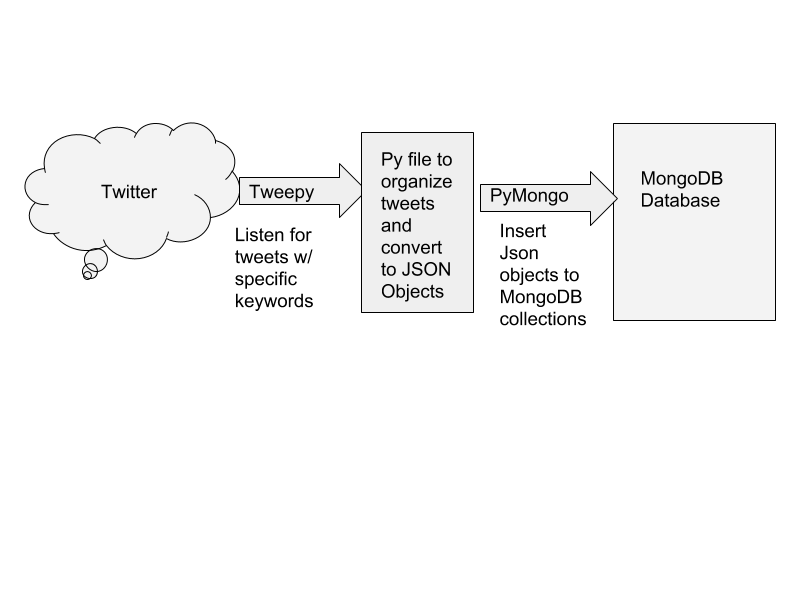
\includegraphics[scale=0.5]{data_collection}
\end{figure}

Building the pipeline consisted of three distinct tasks. 
\begin{enumerate}
	\item Building a tweet streamer to "listen" to tweets based on keywords
	\item Preprocessing the tweets
	\item Storing processed tweets in a database. 
\end{enumerate}
All the code written to built the pipeline can be found in Appendix A.


\section{Streaming Tweets}
\hspace{0.2in} There are two ways to gather tweets using the Python Twitter API (Applications Package Interface). One is to query a profile or a search term. This method is not preferred for several reasons. First, Twitter has put a hard cap on the number of tweets each query can return at one time. This means that querying will be in-exact and time consuming loop. Next, Twitter's search function will naturally promote tweets that have more engagement. This means that tweets with more likes and retweets, comments, and followers will get preference, which results in a biased data set. 

The other way to gather tweets is to stream tweets. A Tweepy stream monitors live twitter content and returns all tweets that contain a given set of keywords. Streaming has the disadvantage of gathering only live tweets - it does not search tweets from before it started running. But, streaming has the advantage of gathering any tweets that meet the keyword requirement, irrelevant of engagement. Consequently, it was decided that the tweets gathered would be through streaming. 

The streamer is abstracted in the Twitter API. To use it, the user must define the actual methods the streamer needs to find and save tweets. The methods defined here are on\_connect, on\_error, and on\_data. The first two are trivial. On\_connect is used to connect, and confirms once the stream is live. If the stream crashes - which can happen for several reasons - on\_error informs the user why the stream stopped (memory, exceeding latency, etc.). The last method on\_data is where the tweets are received and processed. Each tweet is received as a dictionary data structure where keys are attributes of the tweet (i.e. date and time, text, user, etc.). From there any processing is up to the user; the tweet's text can be printed, the tweets can be prepared for entry to a data base, etc. It's here that the tweets will be modified to fit MongoDB's insertion requirements. 

\section{Databases}
\hspace{0.2in} The tweets that the Tweepy streams need to be stored. An Excel file is a convenient but imperfect solution. A database will take full advantage of the object stored as well as the large data set in question. 
\subsection{Overview}
The term database refers to any structure that electronically stores data. In extension, the Database Management System is the program that allows users to interact with the database. In this paper, when the term database is used, it refers to both the structure and the system. 

There are several types of databases. These types are classified by the way the data is organized inside the structure. The relational database model uses tables with rows and columns to store information. Relational databases use SQL to organize, extract, and insert data. Non-relational databases, referred to colloquially to as "NoSQL" use an object-oriented approach with different query languages. 

Databases offer several advantages that other storage options like Excel or CSVs will not. The ability to quickly search and sort through millions of tweets as well as the flexibility to manipulate said data is something that isn't available to Excel. Additionally these databases have organized and maintained APIs for Python. 

\subsection{MongoDB}
\hspace{0.2in} MongoDB is a popular non-relational database management system thats's offered for free. It has an efficient query language as well as a well-defined API Pymongo. In a MongoDB database, each tweet is an object. These objects are stored in collections and the collections are stored in a database:

\begin{figure}[h]
	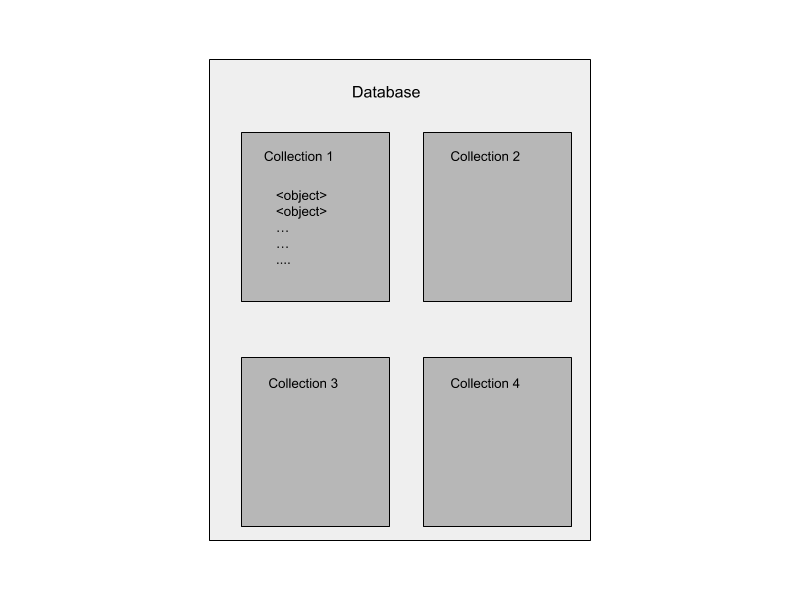
\includegraphics[scale=0.5]{database}
\end{figure}

These JSON objects have fields, populated with values. MongoDB allows a user to query collections using field values. These queries can be exact matches or other operators. For example, you can query tweets by date, or location (by exact match). You can also query sub-matches. That means conditions within a field and not an exact match, like searching for all tweets that contain Donald Trump.

MongoDB has a mongoshell through which a user can interact with the databases. For longer and larger actions, we use the Python API Pymongo to write python scripts. Pymongo allows us to insert, edit, and query databases and manipulate the output. 

For more specifics on Pymongo and setting up MongoDB, refer to the Appendix or the Pymongo documentation.

\section{Data Collection}
\hspace{0.2in} 
Implementing the pipeline referred to earlier means that tweets are streamed and inserted into a MongoDB Database. The first step of streaming requires search terms. These search terms were taken from house and senate races, as well as general terms that refer to the 2018 midterms. Search terms for Senate and House Races were tweets about the candidates as well as a hashtag referring to the race. 

To direct the tweets streamed into a database, the on\_data method is defined. This method is designed for the streamer to deal with the tweets it selects.

\begin{verbatim}
def on_data(self, data):
	try:
            client = MongoClient(MONGO_HOST)

            # Use twitterdb database. If it doesn't exist, it will be created.
            db = client.miscdb

            # Decode the JSON from Twitter
            datajson = json.loads(data)

            #grab the 'created_at' data from the Tweet to use for display
            created_at = datajson['created_at']

            #print out a message to the screen that we have collected a tweet
            print("Tweet collected at " + str(created_at) + " " + datajson['text'])

            #insert the data into the mongoDB into a collection called twitter_search
            #if twitter_search doesn't exist, it will be created.
            db.misc.insert(datajson)
        except Exception as e:
           print(e)
\end{verbatim}

The tweet is converted into a JSON object - MongoDB's preferred type - and inserted into a database and collection of the users choice. This is a barebones definition. Sorting, editing, and adding information to tweets would all be defined here. For the entire script that streamed tweets for the senate or the house, refer to Appendix A.

The data collection process ran through three separate scripts each with a different set of search terms. Those three scripts fed into three different collections in a massive database. Together they assemble a diverse dataset that contains just under three million tweets. Chapter four will explore the dataset we've assembled. 

%%%%% Chapter 3 %%%%%%%%%%%%%%%%%%%
\chapter{Sentiment Analysis}
\label{ch:3}
\hspace{0.2in}Sentiment analysis is the computational approach to evaluating text, which includes determining both sentiment (positive/negative) and intensity. There has always been an interest in the idea of sentiment analysis or objectively evaluating text for polarity. But, the field has seen a burst of activity in recent years due to a few key factors - the availability of text through the world wide web, the advance of big data, and the improvement in machine learning techniques. 

The question of sentiment analysis's real effectiveness is often brought up. The general consensus is that a ceiling does exist for sentiment analysis, much like a ceiling exists for human analysis. There are statements where humans disagree on the sentiment. The ceiling is statements that have near unanimous agreements. If most humans can agree on a statements, it's not a stretch to assume that an algorithm could come to a similar conclusion. 

This paper aims to use sentiment analysis to "poll" twitter users. The model built will make the trade-off specific targeted questions for a large sample size. To make use of collected data, it's important that the sentiment analysis algorithm used is effective and fast; after all, it has to evaluate three million tweets. 

\section{Lexicons}
\hspace{0.2in}The basic idea of sentiment analysis is really simple. The algorithm recognizes positive and negative words, and then finds a method to average these words and determine an overall sentiment and intensity for the statement. But how does it know which words are positive and which words are negative? It uses a lexicon. 

Lexicons are dictionaries. Large dictionaries which contain a list of positive and negative words, each with an intensity expressed. They allow algorithms to quickly ascertain the meaning of a word without having to re-define the word each time. Several well-received lexicons include the LIWC, Bing Lui, and the Harvard Inquirer. The lexicon that we'll use is known as VADER, which will be thoroughly examined later in the chapter. 

Lexicons can be broken into two types - semantic orientation or polarity based, and sentiment intensity or valence based. These general classifications cast a wide net and almost all lexicons fit in one or the other. 

 A well-known polarity-based lexicon is the Linguistic Inquiry and Word Count or LIWC (pronounced "Luke"). LIWC organized words into seventy six categories and has about 900 words that are organized into two categories that are associated with emotion. It's the results of efforts by experts in psychology, sociology and linguistics. It's seen as arguably the best lexicon available, but does not recognize acronyms, abbreviations, or slang. These are all large parts of analyzing social text, and LIWC falls short. 

The original valence-based lexicon is The Affective Norms for English Words or ANEW. It created ratings for over one thousand words of the english dictionary on a scale from one to nine, with a neutral midpoint at five. Words with a value greater than five will have a positive and pleasant meaning and negative and unpleasant otherwise. 

\section{VADER}
\hspace{0.2in}The algorithm used to evaluate the data set is known as the Valence Aware Dictionary for sEntiment Analysis or VADER. It was developed by a pair of researchers CJ Hutto and Eric Gilbert at the Georgia Institute of Technology for the express use of evaluating valence in social media. 

Social media and microblogging in particular poses a challenge to to sentiment analysis algorithms. This is the result of several problems. Earlier lexicons and algorithms were developed before social media's usage rates grew exponentially. They simply cannot handle the rate and volume that social media content is produced. Next, microblogging content is short. Twitter is limited to just two hundred and eighty characters. The average tweet is no more than a sentence or two. This limits context clues for traditional algorithms to pick up. Lastly, social media is famous for its abbreviations. Phrases like "LOL", "IRL", and "TBH" are commonplace on Twitter, but not commonplace on lexicons developed for traditional text. These are problems that VADER solves.

\subsection{Construction}
\hspace{0.2in}Hutto and Gilbert had four goals when they constructed the lexicon and the algorithm:
\begin{enumerate}
	\item The algorithm performs effectively on social media text, but can still be generalized to all media sources. 
	\item The algorithm should have no training required from the user, but should still be based on a human created and cured lexicon. 
	\item The algorithm should be fast enough to use online.
	\item There's no need to make a speed-performance tradeoff. 
\end{enumerate}

A basic overview of the VADER construction process is as follows. Hutto and Gilbert took the LIWC lexicon and made every single term in the lexicon a candidate for a new lexicon. Then, they proceeded to add social media specific terms which include abbreviations, phrases, and emojis as new candidates. These terms were trimmed and weighted in several stages until the final lexicon was produced. 

%Find a source to evaluate Wisdom of the Crowd
The first stage of trimming used Wisdom-of-the-Crowd. WotC uses a large number of people to evaluate words in the lexicon. The large numbers combats the inexperience of the human raters themselves. Terms with a non-zero valence score were eliminated. Terms with a standard deviation greater than 2.5 which indicates that crowd couldn't reach a reasonable consensus were also eliminated. The terms were left had both a sentiment and an intensity. Terms such as "good" and "okay" while both positive, had a difference in score distinguishing their different meanings. 

Their next stage used professional raters to identify parts of texts that can modify intensity despite not necessarily having an intensity themselves. These heuristics includes punctuation, verbal modifiers, and capitalization. Other heuristics identified were terms like "but" that signals a shift in sentiment and negated sentiment. 

The last stage used professional raters to distinguish specific intensity modification of heuristics. This was done by taking a tweet, modifying either the syntax or the punctuation, and then randomly inserting these modifications into the dataset for the raters to evaluate. That way the algorithm could put a score on the change in intensity. 

\subsection{Effectiveness}
\hspace{0.2in} The algorithm's effectiveness can only be evaluated by comparing it to the ground truth. The research team obtained ground truth statements for four domains - social media, movie reviews, product reviews, and editorials. 

VADER's lexicon's competence was compared to several other well known lexicons such as LIWC, Bing Liu, Harvard Inquirer's, and more. This comparison made sure to use the same rule-based model for all of the lexicons. The three factors to evaluate the lexicons were:
\begin{itemize}
	\item The correlation of computed intensity to the ground truth intensity. 
	\item Precision - the number of items correctly classified divided by the number of total items. 
	\item Recall - the number of items correctly classified divided by the number of items in the particular class
	\item F1 Score - the harmonic mean of the precision and the recall.
\end{itemize}

VADER outperformed some of the best lexicons in the industry currently. The results show that VADER's correlation was consistently higher, and it had the best F1 score for tweets. Hutto and Gilbert concluded that the reason was incorporating human heuristics into their model, essentially balancing a quantitative and qualitative approach. 

\subsection{Using VADER}
\hspace{0.2in}VADER was written in Python, and is available to be implemented in Python. Below is how to use VADER to evaluate a single tweet. 
\begin{verbatim}
from vaderSentiment.vaderSentiment import SentimentIntensityAnalyzer

analyzer = SentimentIntensityAnalyzer()
analyzer.polarity_scores("I'm so happy!")
\end{verbatim}
This piece of code will return the following output:
\begin{verbatim}
{'neg': 0.0, 'neu': 0.318, 'pos': 0.682, 'compound': 0.648}
\end{verbatim}
The package returns a series of scores, breaking down how the various components of the model's final score. Positive tweets are tweets that score greater than zero and negative tweets score less than. The intensity is determined the absolute value of the score. 

A few interesting observations to note:
\begin{itemize}
	\item Sarcasm is impossible for the algorithm to understand. To be fair, many humans also struggle with recognizing sarcasm in text.
	\item Any tweet that's an observation tends to be neutral, even if that observation has a positive or negative slant. 
\end{itemize}

\section{Building a Sentiment Profile}
Each candidate in a given race has tweets about them. Using VADER, we can build a sentiment profile for them. The sentiment profile contains five statistics:
\begin{itemize}
	\item Total Number of tweets
	\item Number of Neutral Tweets (Compound = 0)
	\item Number of Positive Tweets (Compound $>$ 0)
	\item Number of Negative Tweets (Compound $<$ 0)
	\item Average Compound Score
\end{itemize}
The sentiment profile will be the base of the features we'll use to model. Below is a snippet of code that calculates the profile for a given user.
\begin{verbatim}
sentiment = analyzer.polarity_scores(tweet) 
if (sentiment['compound'] == 0):        
	neu_tweets += 1          
if (sentiment['compound'] > 0):        
	pos_tweets += 1            
if (sentiment['compound'] < 0):
        	neg_tweets += 1
ave_score += sentiment['compound']
count += 1
\end{verbatim}
This snippet exists in a for loop that iterates through all the tweets found about a candidate. For the full script, refer to the Appendix. 

Here's an example of a sentiment profile:
\begin{center}
\begin{tabular}{ |c|c|c|c|c|c|c|} 
	\hline
	Candidate & Race & Count & Pos Tweets & Neg Tweets & Neu Tweets & Ave Compound\\
 	\hline 
	Ted Cruz & Texas Senate & 111459 & 39642 & 33701 & 38116 & 0.0147602033 \\
  	\hline
	Beto O'Rourke & Texas Senate & 34926 & 11445 & 3830 & 19651 & 0.1143955134 \\ 
	\hline
\end{tabular}
\end{center}
These profiles exist for every single candidate that participated in the election. You can find the sentiment profiles for house and senate candidates in Appendix C. The profiles are the data that will feed into the models that we'll build. 



%%%%%%Chapter 4%%%%%%%%%%%%%%%%%
\chapter{Exploring the Dataset}
\label{ch:4}

\hspace{0.2in}At the end of Chapter \ref{ch:3} we discussed building sentiment profiles for a candidate. These profiles are inspired by the profiles that many polling places create as they ask questions on their candidate. To run with the inspiration, this chapter dives into the dataset that we've created and examines if trends found in polling are reflected on twitter.  

\section{Races Collected}
\hspace{0.2in}In the data gathering process, tweets were collected from thirty-three senate races, twenty nine house races, and a series of miscellaneous hashtags designed to capture national sentiment about the election. 

After counting tweets and more, displayed below are leaderboards for house and senate. The most popular races consisted of the races with the most tweets and engagement. The Most Tweets category refers to the candidates that were tweeted about the most. The Best Liked goes to the candidate that had the highest portion of positive tweets. Least liked and Most Boring work the same way, except for Negative and Neutral tweets respectively. There was a five hundred tweet minimum to qualify for the leaderboard. 
\begin{center}
\begin{tabular}{ |c|c|c|c|c|c|} 
	\hline
	Rank & Most Popular Race & Most Tweets & Best Liked & Least Liked & Most Boring \\
 	\hline 
	1 & Texas Senate & Ted Cruz & Angela Green & Josh Hawley & Tony Campbell\\
  	\hline
	2 & Florida Senate & Rick Scott & Lawrence Zupan & Angus King & Kevin Cramer\\ 
	\hline
	3 & Indiana Senate & John James & John Barasso & Bill Nelson& Matt Rosendale\\
	\hline
\end{tabular}
\end{center}
\begin{center}
\begin{tabular}{ |c|c|c|c|c|c|} 
	\hline
	Rank & Most Popular Race & Most Tweets & Best Liked & Least Liked & Most Boring \\
 	\hline 
	1 & NY-22 & Troy Balderson & Xochitl Small & Josh Hawley & Lizzie Fletcher\\
  	\hline
	2 & VA-07 & Steve Knight & Harley Rouda & Angus King & John Culberson\\ 
	\hline
	3 & KY-06 & Mike Bishop & Ross Spano & Bill Nelson& Gil Cisneros\\
	\hline
\end{tabular}
\end{center}

One interesting point is that those who lead the various sentiment-based categories were no where close to the leaderboard in the most tweets category. Generally it felt that if a candidate was tweeted about more, their average sentiment score tended to drift towards neutral with the positive and negative tweets balancing out. Here is that relationship in graph form. 
\begin{figure}[H]
\centering
	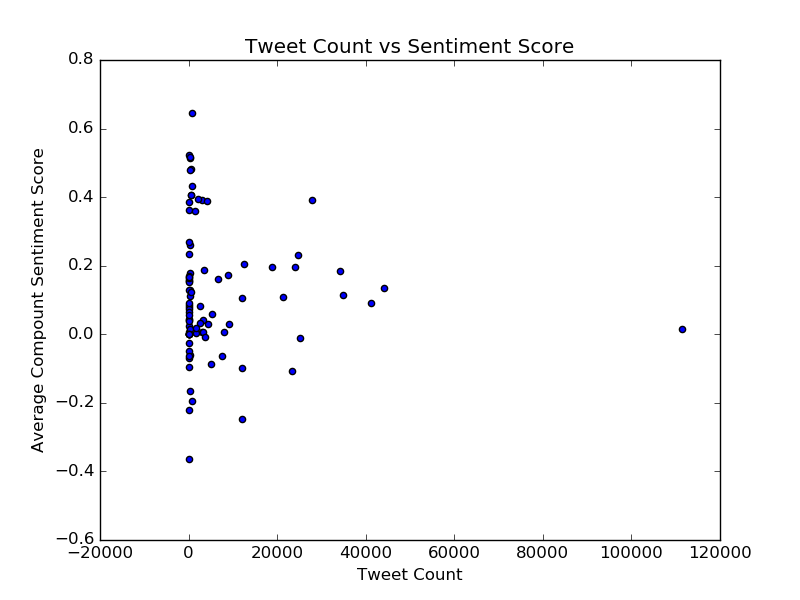
\includegraphics[scale=0.5]{count_sentiment}
\end{figure}
As the count increases, the range in sentiment scores decrease. The samples with tweet counts greater than twenty thousand all stay within a range of 0.4 on either side of neutral. Conversely, the range for sample sizes less than twenty thousand is from -0.4 all the way to 0.7. Essentially, the larger sample sizes are more balanced with a number of positive and negative tweets. That lends support to the idea that our sample isn't overly biased in one ideological direction. 
\section{Comparing Sentiment}

\subsection{Winners vs Losers}
\hspace{0.2in}The point of an election is to win. The question everyone wants to answer is how? What's separates the winners from the losers, and how is that reflected on Twitter? Let's take a look at all the features from the sentiment profiles we created in Chapter \ref{ch:3}. We'll begin with the senate. 

The graph below shows the average compound sentiment score for winning and losing Senate candidates.
\begin{figure}[H]
\centering
	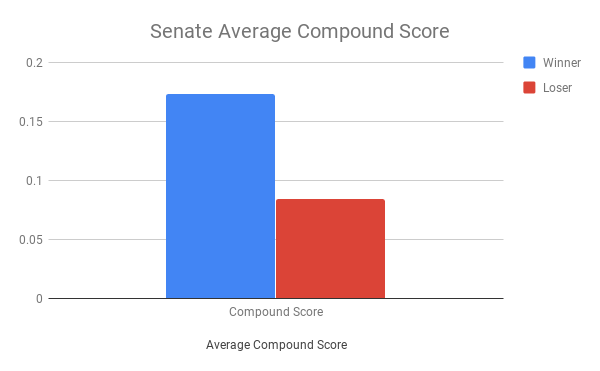
\includegraphics[scale=0.5]{sen_ave_score}
\end{figure}
The winning candidates are heads and shoulders above the losing candidate, and have a much better sentiment score as a whole. That feels right. Candidates that win elections are favored by the voters and that should be reflected on twitter. 

Compound score is a combination of positive and negative tweets. If winners have a higher compound score, it stands to reason that losers will have more negative tweets than winners. The next figure breaks down the count by type of tweet - positive/negative/neutral. 

\begin{figure}[H]
\centering
	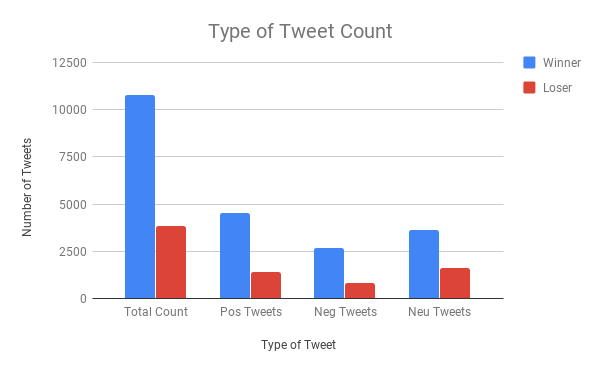
\includegraphics[scale=0.5]{tweet_type}
\end{figure}

The election losers don't actually have fewer negative tweets. That's probably because there's just so many more tweets regarding winners than there are losers. To get a better view, let's break down types of tweets into percentages of the total count. That is to say, what percentage of a winner's tweets are positive, negative, or neutral?

\begin{figure}[H]
\centering
	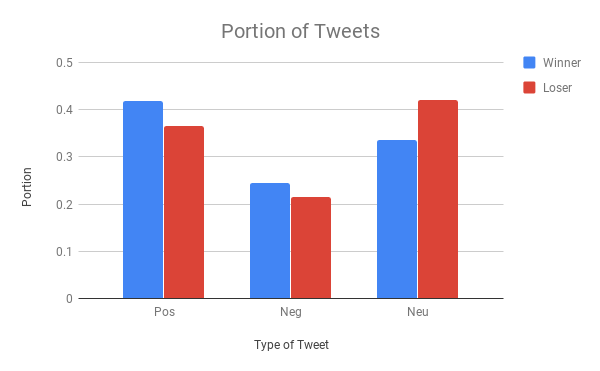
\includegraphics[scale=0.5]{tweet_breakdown}	
\end{figure}

A closer look shows that the real difference lies in the fact that losers have a greater portion of neutral tweets than winners do. In therms of positive and negative tweets, the portions differ by less than five percentage points. Neutral tweets have a sentiment score of zero which would dilute and lower the average compound scores. Winners are not only tweeted about more than losers, but they're more likely to have tweets that show \textit{some} sentiment. But do these patterns hold true for the house?

The average compound scores for winners and losers are displayed below:

\begin{figure}[H]
\centering
	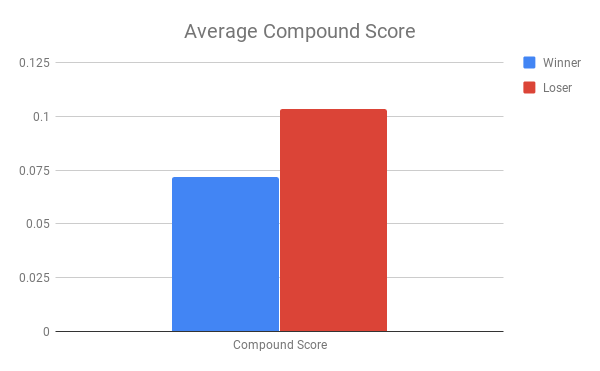
\includegraphics[scale=0.5]{house_compound}
\end{figure}

Unlike the senate, the losers had a higher average sentiment score than the winners. That's unexpected. Let's take a deeper look into how those numbers break down. 

\begin{figure}[H]
\centering
	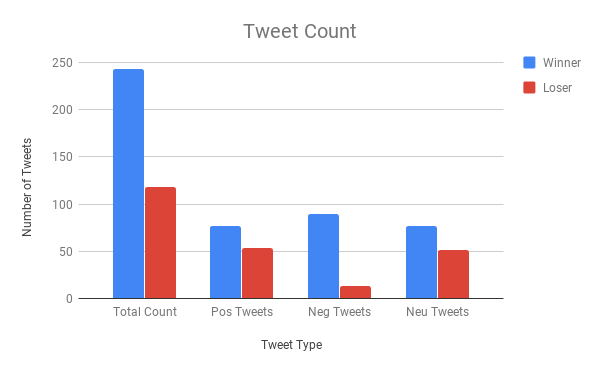
\includegraphics[scale=0.5]{house_tweet_type}
\end{figure}

Winners do have more positive tweets, but the large difference in the number of negative tweets is what ultimately influences the lower average compound score seen. Unlike the senate, the house races show an even-ness when it comes to neutral tweets. These numbers are hardly conclusive, partially because the large difference in tweet count is inflating these numbers. Here's a breakdown of the tweet portions:

\begin{figure}[H]
\centering
	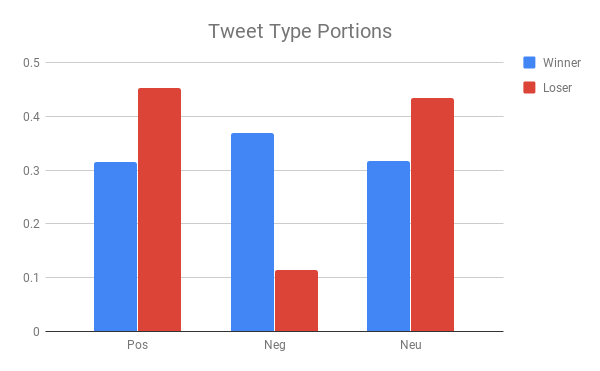
\includegraphics[scale=0.5]{house_tweet_breakdown}
\end{figure}

The house and the senate winners both roughly have 30\% of their tweets designated neutral. The real difference is that negative tweets occupy a far higher proportion of tweets. It doesn't feel that positive and negative tweets have a distinguishable effect on winning. In fact, the only trend that holds across both house and senate winners is the fact that winners are just tweeted about more. The house had a ratio of about 2-to-1 while the senate had 3-to-1. Bottom line, positive tweets are preferred, but overall engagement is key. 

\subsection{Democrats vs Republicans}
The two party system is a large part of our election process. The parties command massive influence and many voters choose a candidate based entirely on party affiliation. This means that a party's national platform and performance can influence their performance in more local elections like the house and the senate. 

In the house, the Democrats flipped a number of Republican Incumbents taking a majority. In the Senate, the Republicans held the majority thanks to the uneven split in seats up for election.

\begin{center}
\begin{tabular}{|c|c|c|}
	\hline
	Incumbents & House & Senate \\
	\hline
	Democrats & 1 & 24\\
	\hline
	Republicans & 28 & 9\\
	\hline
\end{tabular}
\end{center}

\begin{center}
\begin{tabular}{|c|c|c|}
	\hline
	Winners & House & Senate \\
	\hline
	Democrats &  &  \\
	\hline
	Republicans &  &  \\
	\hline
\end{tabular}
\end{center}

In the previous section, it showed that overall sentiment and tweet counts were two features that winners of elections had. If those traits hold, it should show that Democrats in the house should have a higher average sentiment and more tweets and the same for Republicans in the Senate. 

\begin{figure}[H]
\centering
	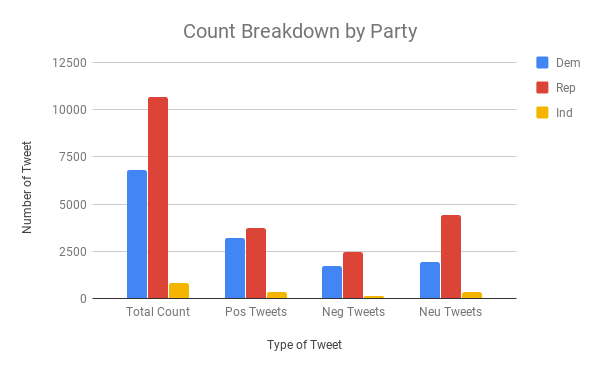
\includegraphics[scale=0.5]{count_party_senate}	
\end{figure}

The Republican dominated Senate did indeed carry the higher total count. They also led in every single other category. This will have interesting effects on the actual sentiment comparison.

\begin{figure}[H]
\centering
	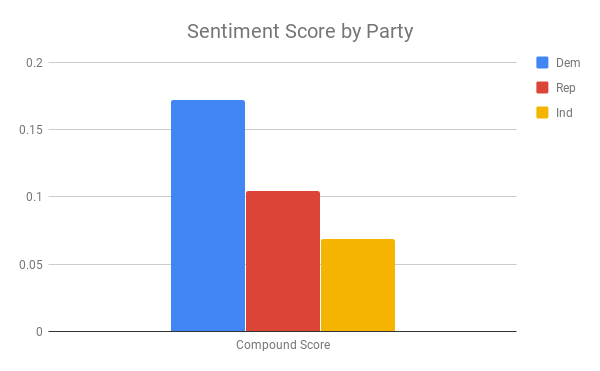
\includegraphics[scale=0.5]{party_sent}
\end{figure}

Republicans leading both in positive and negative tweets meant that they suffered in the overall sentiment tally. The winning party held the tweet count lead, but not overall sentiment. If tweet count is truly the major feature to follow, the trend should hold in the house.

\begin{figure}[H]
\centering
	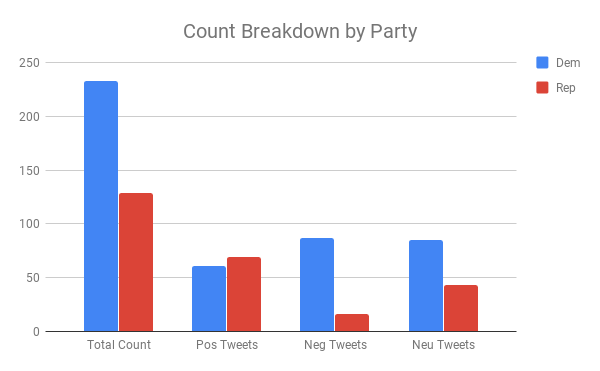
\includegraphics[scale=0.5]{count_party_house}
\end{figure}

\begin{figure}[H]
\centering
	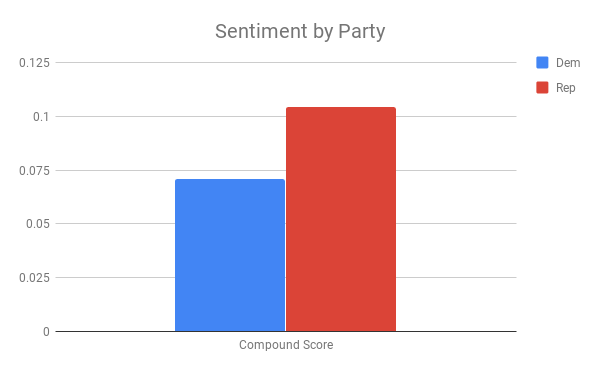
\includegraphics[scale=0.5]{party_sent_house}
\end{figure}

The main takeaway here is that the tweet count lead continues to hold. The sentiment score favors the Republicans - the losing party - but that correlates with the fact that losing candidates in the house had a better sentiment score as well. 

\section{National Trends}
\hspace{0.2in} This data set presents the opportunity to explore how national trends are reflected on twitter. Not only that, it'll give a better idea on the kind of sample collected and how it reflects to the samples pollsters take when they observe overall trends they expect to influence elections. 

Eight search terms were used to create a database of miscellaneous tweets. These search terms were largely national trends:

\begin{figure}[H]
	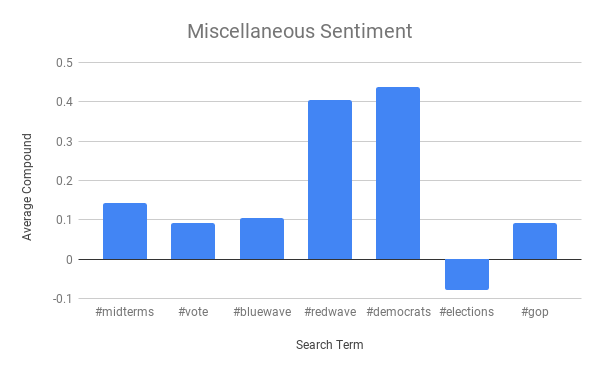
\includegraphics[scale=0.5]{misc_sent}
\end{figure}

The sentiment of partisan search terms are about the same. Non-partisan terms have sentiments within a similar range with the peculiar exception of ``\#elections". The purpose of this exercise was to show that this database is mostly neutral in contrast to the house leaning democrat and the senate republican. 

The three major trends we're examining are sourced from an ABC news article published on November 6th. The article identified health care, border security, and Donald Trump as three major factors heading into the midterm election.

\subsection{Exploring the Issues}
\label{subsec:exploring the issues}
\hspace{0.2in}The main motivation for this project \textit{was} Donald Trump. Mr. Trump was a controversial candidate and is now a controversial president. The midterms are often considered a referendum against the president. Areas which view Mr. Trump favorably should lean republican while those who don't favor him should lean democrat. Since taking office, Mr. Trump has averaged a favorability rating of forty percent while never being higher than forty-five. 

Health care has had an interesting history in US Politics. In 2010, President Barack Obama passed the Affordable Care Act allowing access for millions of uninsured. Despite many Republican efforts, including a late push by congress in 2018, the ACA still stands. Several moderate Republicans avoided voting against it due to its popularity in their district/state. 

According to the Kaiser Family Foundation, the ACA continues to remain a hot topic among voters. A different Pew Research poll showed that sixty percent of voters believe that health care is the government's responsibility. 

The last major issue is the border wall. Mr. Trump's first campaign promise was the wall and his continued attacks on illegal immigration gained him significant support. After taking office, Mr. Trump has wielded the Immigrations and Customs Enforcement Division (ICE pronounced "ice") as a baton to round up and deport illegal immigrants. A gallup poll had just twenty percent of respondents view Illegal Immigration as ``not a problem". 

These three issues are front and center, and the data set should have views about them. Having Twitter's numbers agree in some form with that of traditional pollsters shows that the data set is a fair representation of the populace. 

\subsection{Evaluating Twitter's Response}
\hspace{0.2in}There were six search terms taken from the three issues. Using modified code that can be found in Appendix B, a sentiment profile was put together. Each term was searched independently in the senate, house, and miscellaneous database. The goal was to have the three databases capture a different type of population. 
\begin{figure}[H]
	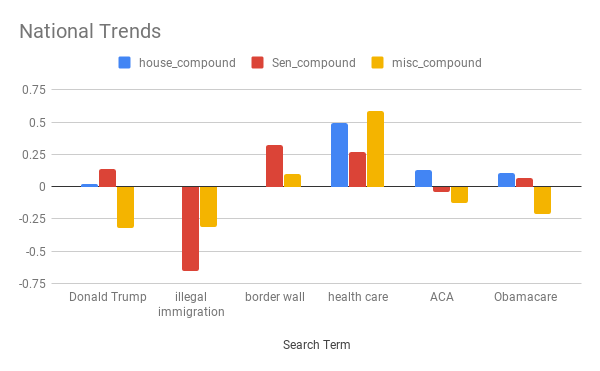
\includegraphics[scale=0.65]{natty_trends}	
	\caption{Sentiment scores of search terms that describe important national trends}
	\label{fig:natty_trends}
\end{figure}

Looking at Figure \ref{fig:natty_trends} that assumption holds up. Mr. Trump is viewed favorably in the Republican dominated Senate, while less so in the house and in general. His house sentiment may be a result of a majority of house elections had republican incumbents. His intense negative sentiment with the general populace correlates with that of his general favorability - which is below average. 

On illegal immigration, it's interesting to see that Democrats took no stance. That could be because if they did, they would be in the minority. Sentiment is decidedly against illegal immigration and very much for the border wall. This is not only in the republican-dominated Senate but in the more neutral miscellaneous database. It's possible that Democrats saw a path through success by simply not addressing illegal immigration and focusing on other topics that were in their favor like health care. 

In section \ref{subsec:exploring the issues} a Pew research poll was referenced regarding health care and the government. Specifically voters believed that health care was a governmental responsibility. They've echoed that sentiment here, as big fans of health care as an idea in general, but not of specifically the ACA. Notice that the ACA and Obamacare reference the same piece of legislation, but Obamacare's sentiment is noticeably lower in all three categories. That may be because of the vitriol Obama faces by Republicans and even the nation. It's clear that Obama's controversial presidency is still showing effects. So much so, that just the name on the paper makes all the difference.  

%%%%%Chapter 5%%%%%%%%%%%%%%%%%%%
\chapter{Modeling Elections}
\label{ch:modeling}
hspace{0.2in}The goal of this project is to build a model that will predict elections. Every part of the previous chapters were a build up to create a model. Data has been collected, cleaned, and organized. Tweets have been evaluated with VADER. This chapter will cover the model building and the results from the model. 

\section{Approach}
\hspace{0.2in}Part of planning and designing a model is an understanding of the model's purpose. What is the model going to do? Will it make a decision? A recommendation? These are questions that will determine the type and effectiveness of the model that's built. 

The challenge with elections is that they are a zero-sum game. When a candidate wins an election, the other candidate loses. The approach taken is to remove the game entirely. Rather than focus on an election the model will focus on a candidate, and act as if they exist in a vacuum. It will predict a candidate's chances of winning their election independent of the other candidates' own probability. That means that the sum of the winning probabilities for all candidates in a given election is not always 1.

This approach will challenge the model constructing portion. This is a shift away from using the tweets as express data input. It's instead a higher-level approach. We will use the summary statistics per candidate as input instead. 

\section{A Machine Learning Overview}
\hspace{0.2in} The layman's definition of machine learning is to ``program a computer to accomplish a task that you don't know how to do''. Most coding is to explicitly define a task. Machine learning offers the ability to teach an algorithm the rules of the task, and then allow the algorithm to find its own method to accomplish it. There are many subfields, but the type of learning we'll focus on is supervised learning. 

Supervised learning is a type of learning where an algorithm is given input, output pairs and uses those pairs to infer the function. To put it more simply, we give the algorithm both the question and the answer, and it finds out the method to solve it. When creating a supervised learning model, it will need to be trained and tested. A full set of data is split into training and testing sets. The model will use the training set to create the best map it can. The testing set evaluates the map's effectiveness. 

A clean, extensive, and unbiased data set is crucial to a successful supervised learning model. The maps that the model creates is reliant entirely on data. A biased dataset will result in a biased model. A few examples of supervised learning include linear and logistic regression, perceptron learning, and naive bayes. 

The specific problem in question is a binomial classification problem. Each input has two potential results - winning or losing. With binomial classification, there are a variety of models available. Due to a variety of reasons that will be thoroughly examined in the next section, we've chosen to proceed with the Naive Bayes Classifier, a machine learning technique based on Bayes Theorem of Conditional Probability. 

\section{Understanding the Naive Bayes Classifier}
\hspace{0.2in} The Naive Bayes classifier is a Bayesian classifier. All Bayesian classifiers are decision making systems that are based off of Bayes Theorem of Conditional Probability. Bayes Theorem makes a prediction based on observation. 

Given that you have an object with feature $A$ and a class $B$, the probability that the object belongs to class $B$ based on observation $A$ is:
\begin{equation}
\label{eq:bayes}
P(A|B) = \dfrac{P(B|A)P(A)}{P(B)}
\end{equation}

A Bayesian classifier uses that theorem and extends it to make a prediction. Imagine that there are classes $A$ and $B$ and an object with observation $x$. 
\begin{figure}[H]
\centering
	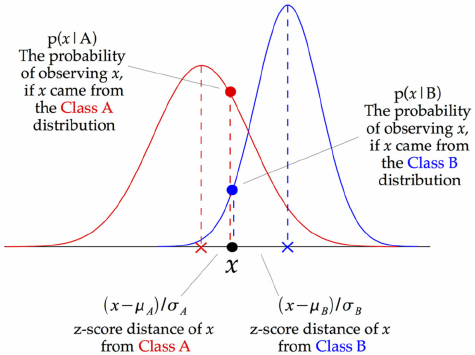
\includegraphics[scale=0.5]{bayes}
\end{figure}
The classifier uses Bayes Theorem, calculates $P(x|A)$ and $P(x|B)$ before making a decision based on the resulting probabilities. This example used one observation with two classes. What happens in the case where you have more than one observation? That's the problem the Naive Bayes classifier solves. 

The classifier assumes that each parameter is independent from the other. Given a set of observations $d$ and a class $c_j$, the probability that $d$ came from $c_j$ is:
\begin{equation}
\label{eq:naivebayes}
P(d|c_j) = P(d_1|c_j) \cdot P(d_2|c_j) \cdot \ldots \cdot P(d_n|c_j)
\end{equation}
which can be simplified to:
\begin{equation}
\label{eq:simnaivebayes}
P(d|c_j) = \prod^{n}_{i=1} P(d_i|c_j)
\end{equation}
This process repeats for all possible classes and the decision is the class with the highest probability. Thus we obtain the following classification rule:
\begin{equation}
\label{eq:classrule}
P(c_j | d_1,\dots,d_n) \propto P(c_j) \prod^{n}_{i=1} P(d_i | c_j) \implies \hat{c} = arg\max_{c_j}P(c_j)\prod^{n}_{i=1}P(d_i | c_j)
\end{equation}
This rule determines the class $\hat{c}$ by choosing the class that maximizes probability. In this particular case, those classes are winning and losing an election. 

There are several types of Naive Bayes classifiers. The one that we employed is the Guassian Naive Bayes. It's designed for models where the parameters have continuous input. Using this model changes the way we calculate the conditional probability. With continuous input, we assume the probability to lie on a normal distribution. Keeping the same terminology as equation \ref{eq:naivebayes} we find $P(d_i | c_j)$ as such:
\begin{equation}
\label{eq:gaussprob}
P(d_i | c_j) = \dfrac{1}{\sqrt{2\pi\sigma^{2}_{c_j}}}\exp\left(\dfrac{(d_i - \mu_{c_j})^2}{2\sigma^{2}_{c_j}}\right)
\end{equation}
The parameters $\sigma_{c_j}$ and $\mu_{c_j}$ are estimated using maximum likelihood. 

The Naive Bayes is the optimal solution given the constraints of the problem. First, the classification problem means that the optimal solution is either a neural network, logistic regression, or Naive Bayes. The chosen approach has limited the size of our dataset. Instead of the three million tweets, the inputs are the hundred and fifty candidates. For smaller data sets, the Naive Bayes has been shown to outperform other models. Both regression and a neural network in crude terms weight their parameters to produce a final result. To ensure accurate weights, the training data needs to be extensive, something not available to us currently. The Naive Bayes probability based approach will take advantage of an unbiased dataset regardless of its size. 

\section{Implementation Naive Bayes in Python}
\hspace{0.2in}The python library Sci-Kit Learn contains a variety of machine learning models. The machine learning can be imported from Sci-Kit, fitted with training data, and then tested using their predict method. Importing the library is done through the import statement.
\begin{verbatim}
from sklearn.naive_bayes import GuassianNB
\end{verbatim}

The data to train and test the algorithm needs to be imported, split, and organized before any fitting can happen. The dataset has been stored as a CSV, and the pandas package will make importing and organization easy. They are stored in a dataframe, which is a python object that is similar to an excel table. 
\begin{verbatim}
import pandas as pd

pd.read_csv(FILE_NAME)
\end{verbatim}

The dataframe is sliced into data and labels. Data is the parameters that the algorithm will read and weight. These parameters include Tweet Count, Positive Tweets, Average Compound Sentiment Score, etc. Labels are the answers for the algorithm to check itself against. Did the candidate win or lose. To allow the algorithm to process the label, winning is a 1 and losing is a 0. Both the training and testing sets have a data and label variable. 
\begin{verbatim}
train_data = np.asarray(senate.loc[:70, `Count':`Average Compound'])
train_labels = np.asarray(senate.loc[70:, `Winner')])
\end{verbatim}
You'll notice that the inputs to the algorithm are all arrays of integers. Even when dealing with text, data needs to be tokenized or shaped into integers that can be organized into arrays for the algorithm to process. Shaping the information and then understanding the output is on the user. 

Fitting the algorithm is easy. The gaussianNB object has a fit function that takes the training data and labels as input.
\begin{verbatim}
gnb = GaussianNB()
gnb.fit(train.data, train.labels)
\end{verbatim}

The algorithm is now trained. To evaluate, use the predict function on the testing set. The predict function will output the prediction, and not the conditional probabilities. To see those, use the predict\_proba function. 
\begin{verbatim}
output = gnb.predict(test_data)
probs = gnb.predict_proba(test_data)
\end{verbatim}
With the ability to predict, we can now evaluate the effectiveness of Naive Bayes. 
 
\section{Evaluating the Model}
\hspace{0.2in} Evaluating a model with just accuracy doesn't capture the full picture of how effective a machine learning model is. It is important to examine subsets of the results to understand how the model interacts with specific classifications. To do this, we use the confusion matrix. 

\begin{figure}[H]
\label{fig:confmatrix}
\centering
	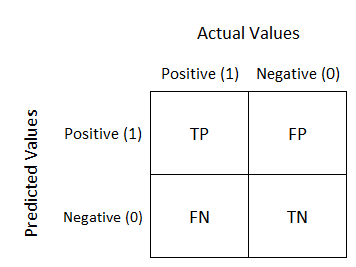
\includegraphics[scale=0.5]{confusion_matrix}
\end{figure}

The confusion matrix outlines the four potential outcomes for any prediction - true/false positives and true/false negatives. These have been used in the medical field for decades when assessing false positives, and gained popularity in machine learning in the 1980's. 

\subsection{Criteria}
\label{subsec:criteria}
\hspace{0.2in} The confusion matrix provides the base for four criteria to evaluate the model. These are precision, accuracy, recall, and f1.

Precision is the ratio of true positives to the sum of true positives and false positives. This is a metric of how often the model is right given that it predicts a candidate to win. It's an important metric because it evaluates the power of the model in regards to predicting a winner. 

\begin{equation}
\label{eq:precision}
PRECISION = \dfrac{TP}{TP+FP}
\end{equation}

Recall is the ratio of true positives to the sum of true positives and false negatives. It's a good measure of how well the algorithm covers actual positive values. 

\begin{equation}
\label{eq:recall}
RECALL = \dfrac{TP}{TP+FN}
\end{equation}

Accuracy is the ratio of true positives to total items in the test set, It's an overall measure of how good the model is. On it's own it's an incomplete metric, but it fits in quite well with the other four. 

\begin{equation}
\label{eq:accuracy}
ACCURACY = \dfrac{TP+TN}{TP+TN+FP+FN}
\end{equation}

Last, the f1 score is the weighted average of the precision and recall. It takes false positives and false negatives into account. 

\begin{equation}
\label{eq:f1}
F1 = 2 \cdot \dfrac{PR \cdot RE}{PR + RE}
\end{equation}

\subsection{Performance}
\hspace{0.2in} To test the model, the data is split into training and testing. First the rows are shuffled and then 75\% of the data goes to training while the other 25\% goes to testing. Here is the resulting confusion matrix from that aplit:
\begin{center}
\begin{tabular}{|c|c|c|}
	\hline
	Predicted/Actual & Positive & Negative \\
	\hline
	Positive & 3 & 8 \\
	\hline
	Negative & 1 &  26\\
	\hline
\end{tabular}
\end{center}
From those, we can calculate the metrics outlined in Section \ref{subsec:criteria}:
\begin{center}
\begin{tabular}{|c|c|}
	\hline
	Metric & Score \\
	\hline
	Precision & 0.75 \\
	\hline
	Accuracy & 0.763\\
	\hline
	Recall & 0.33 \\
	\hline
	F1 & 0.458 \\
	\hline
\end{tabular}
\end{center}

These results are encouraging - particularly the positive precision. Essentially, when the model does decide to predict a positive result, it is likely to be right. It's clear that the model we've implemented is conservative. The significant number of false negatives combine with the low number of false positives shows that the model only predicts positive when a significant amount of evidence shows it to be true. 

The weak recall is potentially a reaction to class imbalance. The negative prediction rate is 0.76. If a larger test set with better balance was included, the greater number of true positives would push the recall higher. 

%%%%%%%Chapter 6%%%%%%%%%%%%%%%%%
\chapter{Conclusion}
\section{Project Achievements}
In the introduction, this project set out to create a model that predicts the outcome of the election. It did accomplish that, predicting elections at a 76\% rate. The end to end project leveraged a number of technologies such as MongoDB, the Twitter API, Python and Sci-Kit Learn, and more. It was a great experiment in understanding and immediately applying new technologies, and has laid the groundwork for expansion come future elections. 

\section{Future Work}
\hspace{0.2in} This project was challenged by the lack of data. Over three million tweets were collected, but those tweets weren't used as individual data points. This project will be improved with more races and candidates collected. The time constraints in November limited the number of races that were followed, but now the data collection pipeline is in place, and all four hundred and fifty races can be followed in 2020. As more races and data is added, the accuracy and effectiveness of the model increase. The larger data set also provides more options as far as model selection such as logistic regression, neural networks, and more. 

This project was a first investigatory effort into the problem of election prediction. There are a variety of factors that haven't been taken into account - such as bots, attacks, and separation of constituencies. More complex models with more data could motivates the potential of further research. 

%%%%% Appendices %%%%%%%%%%%%%%%%%%
\begin{appendices}
%%%%% Appendix A  %%%%%%%%%%%%%%%%%%
\chapter{The How-To Guide}
\hspace{0.2in}The following chapter is an instruction guide to apply the scripts from Appendix B and recreate various parts of the project. If you're looking for full scripts, those can be found in Appendix B. A quick disclaimer. All the instructions that follow are assuming that you are working on a UNIX system such as MacOS or Ubuntu.  

\section{Installation}
\label{sec:install}
There are several programs and packages that need to be installed to gather tweets as well as running a model:
\begin{itemize}
	\item Python3 - If you're working on a UNIX system, this should come pre-installed. If it doesn't, install it using your system's package installation manager. 
	\item MongoDB - A database management system. Find the distribution for your operating system on the website. 
	\item Text Editor - Choose one that best meets your needs. 
\end{itemize}
\newpage
There are several python libraries that need to be installed for the scripts in Appendix B to work. They're listed below:
\begin{itemize}
	\item Tweepy - The Twitter Python API
	\item Pymongo - The MongoDB Python API
	\item vaderSentiment - The python library that contains the VADER algorithm discussed in Chapter \ref{ch:3} 
	\item Sci-Kit - A Machine Learning Library used to build machine learning. models
	\item ConfigParser - A python package used to read and parse through configuration files
\end{itemize}
Python libraries are installed using pip. From the command line, execute the command: \begin{verbatim} pip3 install <library> \end{verbatim}

\section{Gathering Tweets}
\label{sec:collectingtweets}
Once everything from section \ref{sec:install} is installed on your machine, use the following steps to stream tweets into a database:
\begin{enumerate}
	\item Create a developer account on Twitter and create an Twitter application through it. The instructions to do so are provided on https://developer.twitter.com/. Once the application is created, it will provide you with an API Key/Secret Pair. It will also provide you with a token key/secret pair. These four randomly generated strings are how the script will interact with twitter. 
	
	\item Copy and paste the Listener script from Appendix B. Replace the ckey, csecret, atoken, asecret values with your two key/secret pairs. If you'd like to change the name of the database, rename the db variable in the on\_data method. 
	
	\item Before we can run the script, mongodb has to be ready to receive the tweets. Start the mongod daemon from the command line using the command:
	\begin{verbatim}
	$sudo mongod
	\end{verbatim}
	Now, open another tab on the command line and run the script using the command:
	\begin{verbatim}
	$python3 misc_listener.py
	\end{verbatim}
	
	\item To check if the stream is working do the following:
	\begin{enumerate}
		\item Open a new tab in the command line and start the mongo shell with the command:
		\begin{verbatim}
		$mongo
		\end{verbatim}
		\item In the mongo shell use the command:
		\begin{verbatim}
		>show dbs
		\end{verbatim}
		That will output a list of the databases on the server currently. The db name from the script should be listed. 
		\item To see the individual tweets in the database, use the following two commands in sequence. Replace db\_name with the name of your database in the use command :
		\begin{verbatim}
		>use <db_name>
		>db.stats()
		\end{verbatim}
		The stats command will give you an overview of the database. One of the metrics is the number of objects. While the streamer is running, refresh the db.stats() command and observe the object count rising. 
	\end{enumerate}
\end{enumerate}

\section{Building Datasets and Models}
\hspace{0.2in} For this portion, there's little step by step guidance in terms of setup. In Appendix B instructions are included in regards to installation or set up. For any script that's building a sentiment profile or a dataset, the mongod daemon needs to be running. For scripts that are modeling such as naive\_bayes.py, the csv needs to be in the same directory as the script is running from. Those instructions are re-iterated in Appendix B. 

%%%%% Appendix B %%%%%%%%%%%%%%%%%%
\chapter{Code}
This project required a number of python scripts to be written. These scripts covered collecting data, organizing and cleaning collected data, as well as building predictive models. Below, you'll find every script written along with its intended purpose.

\centerline{***}

\textbf{Name:} Listener

\textbf{Purpose:} This script is a filled in template of the code written to stream tweets into a database. The ``misc'' in the title refers to the fact that this version of the script is streaming tweets from the list of miscellaneous search terms. It has two very similar scripts for the senate and the house. 

\textbf{Execution:} It requires a server with the mongod daemon running as well as a Twitter Application with an API key/secret pair. Python packages used are Tweepy and Pymongo. Can be run directly from the command line or through an IDE. Explicit instructions are in Appendix \ref{sec:collectingtweets} 

\textbf{Expected Output:} Will print tweets as they are streamed. Tweets themselves will be stored in the targeted database. 

\lstinputlisting[language=Python]{misc_listener.py}

\newpage

\textbf{Name:} Sentiment Profile

\textbf{Purpose:} This code creates a sentiment profile for a given search term and a given database. The sentiment profile is the same profile that's discussed at the end of Chapter \ref{ch:3}

\textbf{Execution:} This code was written under the assumption that a mongodb database is set up with data looking for. You'll also need vaderSentiment and Pymongo installed through pip. The script is executed from the command line using the following template:
\begin{verbatim}
$python3 sentiment_profile.py <politician> <database>
\end{verbatim}

\textbf{Expected Output:} The output will be a sentiment profile printed to the console:
\begin{verbatim}
	Search Term: Claire McCaskill Race: Missouri Senate Count: 27940 \newline 
	Pos Tweets: 23663 Neg Tweets: 2328 Neu Tweets: 1949 Average Compound: 0.392
\end{verbatim}

\lstinputlisting[language=Python]{sentiment_profile.py}

\textbf{Name:} Build Search Profile

\textbf{Purpose:} This script takes a list of all the races and search terms and creates a sentiment profile to each one and then writes that sentiment profile to a file. That allows use that file for analysis any which way we like. 

\textbf{Execution:} This script needs an accompanying configuration file. That means that you'll also need the Python library ConfigParser to read that configuration file. The other requirements are the same as those required by the Sentiment Profile script. To run the script, use the command:
\begin{verbatim}
	python3 build_search_profile.py senate
\end{verbatim}
To build the profile for the house, use house as the input instead of senate with the same command format as above. 

\textbf{Expected Output:} The file prints whichever race it's currently working on to the console. The final output will be a .csv file it creates in the working directory. 

\lstinputlisting[language=Python]{build_search_profile.py}

\textbf{Name:} Naive-Bayes Modelling

\textbf{Purpose:} The script models a candidate's probability of winning given their sentiment profile. It reads in the data from a given csv, splits the data into training and testing sets, and then trains the algorithm. The script then predicts a series of outputs given the testing set, and then calculates the error. 

\textbf{Execution:} Running this will need the python libraries Sci-Kit Learn or sklearn, pandas, and numpy. It will also need the sentiment profiles that were created from the previous scripts

\textbf{Expected Output:} The script will print out the accuracy of the model to the console. It can be toggled with to print the output as well as the probabilities for the output (bayesian modeling returns a probability of being 1 or 0). 

\lstinputlisting[language=Python]{naive_bayes.py}


\end{appendices}


\bibliographystyle{plain}
\bibliography{midwaybib}
\end{document}